% ============================================================================
%  Undergraduate Thesis — Ingeniería Civil Informática, Universidad Andrés Bello
%  Heuristic Approaches for the k-Traveling Salesman Problem
%  Author: Nicolás Barrientos   Advisor: Dr. Gustavo Gatica
%  Written in English. Compiles in Overleaf (pdfLaTeX).
% ============================================================================
\documentclass[12pt,a4paper,oneside]{report}

\usepackage[utf8]{inputenc}
\usepackage[T1]{fontenc}
\usepackage[english]{babel}
\usepackage[margin=2.5cm]{geometry}
\usepackage{graphicx}
\usepackage{amsmath,amssymb,amsfonts}
\usepackage{booktabs}
\usepackage{tabularx}
\usepackage{array}
\usepackage{caption}
\usepackage{float}
\usepackage[ruled,vlined,linesnumbered]{algorithm2e}
\usepackage{enumitem}
\usepackage{setspace}
\usepackage{url}
\usepackage[hidelinks]{hyperref}
\usepackage{lmodern}

\onehalfspacing
\graphicspath{{.}{./}}
\captionsetup{font=small,labelfont=bf}
\renewcommand{\arraystretch}{1.15}

\begin{document}

% ======================= TITLE PAGE =======================
\begin{titlepage}
\centering
\vspace*{1.5cm}
{\Large \textbf{UNIVERSIDAD ANDRÉS BELLO}}\\[0.2cm]
{\large Faculty of Engineering}\\
{\large School of Computer Engineering (Ingeniería Civil Informática)}\\[3cm]

{\LARGE \bfseries Heuristic Approaches for the\\[0.2cm]
$k$-Traveling Salesman Problem:\\[0.2cm]
A Reproducible Comparison\par}
\vspace{2.5cm}

{\large Thesis submitted in partial fulfillment of the requirements\\ for the degree of Computer Engineer}\\[2.5cm]

\begin{flushright}
\begin{minipage}{0.6\textwidth}
\textbf{Author:}\\ Nicolás Barrientos\\[0.6cm]
\textbf{Advisor:}\\ Dr.\ Gustavo Gatica\\
\end{minipage}
\end{flushright}
\vfill
{\large Santiago de Chile, 2026}
\end{titlepage}

% ======================= COPYRIGHT =======================
\thispagestyle{empty}
\vspace*{\fill}
\begin{center}
\textbf{Copyright}
\end{center}
\noindent
\copyright\ 2026, Nicolás Barrientos. All rights reserved.

\vspace{0.4cm}
\noindent
Total or partial reproduction of this work, by any means or process, is
authorized only for academic purposes, provided that the source is
acknowledged and the corresponding credit is given to the author and to
Universidad Andrés Bello. Any use for commercial purposes requires the
express written permission of the author.
\vspace*{\fill}
\clearpage

% ======================= ACKNOWLEDGMENTS / DEDICATION =======================
\chapter*{Acknowledgments and Dedication}
\addcontentsline{toc}{chapter}{Acknowledgments and Dedication}

I would like to thank my advisor, Dr.\ Gustavo Gatica, for his continuous
guidance, patience, and technical insight throughout the development of this
work. I am also grateful to the co-authors and reviewers whose comments
substantially improved the quality of the study, and to Universidad Andrés
Bello for the academic environment that made this research possible.

\vspace{0.5cm}
\noindent
This work is dedicated to my family, whose constant support and encouragement
have accompanied me throughout my studies.

\clearpage

% ======================= DECLARATION ON THE USE OF AI =======================
\chapter*{Declaration on the Use of Artificial Intelligence}
\addcontentsline{toc}{chapter}{Declaration on the Use of Artificial Intelligence}

In accordance with the academic integrity guidelines of Universidad Andrés
Bello, I declare that generative artificial intelligence tools were used during
the preparation of this thesis in a supporting and auxiliary role only. Their
use was limited to: assistance with the wording and English style of the text,
help organizing the document structure, support in debugging and documenting
source code, and the generation of figures from data that were produced by the
author's own experiments.

All the scientific content of this thesis --- the mathematical formulation, the
design and implementation of the algorithms, the experimental protocol, the
data, the results, and the conclusions --- is the author's own work. Every
numerical result reported here was obtained by executing the author's code on
standard TSPLIB instances, and the reference (best-known) values were computed
with the official LKH-3 solver. The author takes full responsibility for the
content of this document.

\clearpage

% ======================= ABSTRACT =======================
\chapter*{Abstract}
\addcontentsline{toc}{chapter}{Abstract}

The $k$-Traveling Salesman Problem ($k$-TSP) is a variant of the classical
Traveling Salesman Problem in which, given $n$ cities that include a home city
(depot) and a fixed value $k$ with $1<k\le n$, one seeks a single closed tour of
minimum total length that starts and ends at the depot and visits exactly $k$
cities. Solving it therefore involves two coupled decisions: \emph{which} $k$
cities to visit and \emph{in which order}. This dual nature distinguishes the
$k$-TSP from the standard TSP and is the source of its combinatorial difficulty.

This thesis presents a reproducible repository and an experimental comparison of
\textbf{ten} solution techniques for the $k$-TSP: a greedy cheapest-insertion
heuristic, a GRASP/multi-start scheme, a genetic algorithm, the classical Nearest
Neighbor and the Nearest, Farthest and Random Insertion construction heuristics,
Simulated Annealing, Tabu Search, and the proposed deterministic heuristic
\textbf{DCIH} (Deterministic Cheapest-Insertion Heuristic). As the reference for
solution quality, the best-known values (BKS) obtained by the
Lin--Kernighan--Helsgaun solver (LKH-3) on the benchmark instances of Pandiri \&
Singh are used. Experiments on 38 standard TSPLIB instances, across three values
of $k$ ($\approx n/4$, $n/2$, $3n/4$), evaluate solution quality (relative GAP)
and, following Weise \textit{et~al.}, the \emph{anytime} behavior of the methods
through progress curves, ECDF, estimated running time (ERT) and an aggregated
global ranking on a machine-independent time axis.

The results show that the greedy cheapest-insertion baseline and Tabu Search
attain the lowest average GAP overall, with Tabu Search the best of the
metaheuristics; that the genetic algorithm becomes the most frequent per-instance
winner for large $k$; that Farthest Insertion is the weakest method because
selecting distant nodes conflicts with the node-selection objective; and that the
proposed DCIH offers a deterministic, fully reproducible alternative of
comparable quality.

\vspace{0.3cm}
\noindent\textbf{Keywords:} $k$-TSP, greedy heuristics, GRASP, genetic algorithms,
simulated annealing, tabu search, Lin--Kernighan--Helsgaun, anytime benchmarking,
TSPLIB.

\clearpage

% ======================= TABLE OF CONTENTS =======================
\tableofcontents
\clearpage

% ============================================================================
%  CHAPTER 1 — CONTEXT AND OBJECTIVES
% ============================================================================
\chapter{Context and Objectives}

\section{Context}
Route optimization is one of the most studied problems in operations research
and computer science because of its direct impact on logistics, transportation,
surveillance and resource planning. The Traveling Salesman Problem (TSP) --- the
task of finding a minimum-length closed tour that visits every city exactly once
--- is the canonical representative of this family and a reference benchmark for
combinatorial optimization.

Many real applications, however, do not require visiting \emph{all} the available
locations. When a fleet, a courier or a sensor must serve only a subset of the
sites under a budget on the number of stops, the appropriate model is the
\textbf{$k$-Traveling Salesman Problem} ($k$-TSP): given $n$ cities including a
depot and a fixed value $k$ with $1<k\le n$, find a single closed tour of minimum
total length that starts and ends at the depot and visits exactly $k$ cities,
chosen from the $n$ available. Unlike the classical TSP, the $k$-TSP couples two
decisions --- \emph{which} $k$ nodes to visit and \emph{in which order} --- and
this selection-plus-ordering nature is what makes it combinatorially hard: the
number of candidate subsets alone is $\binom{n-1}{k-1}$, and each admits
$(k-1)!/2$ distinct tours, so exhaustive enumeration is intractable already for
medium-sized instances.

The $k$-TSP belongs to the broader family of \emph{TSP with profits} and
selective routing problems, which includes the Orienteering Problem and the
Prize-Collecting TSP. It models, for instance, selective sampling, prize- or
quota-collecting routing, surveillance with a limited number of visits, and
resource-constrained logistics, where solving the problem well translates
directly into lower cost and better resource utilization. This practical
relevance, together with the scarcity of reproducible experimental comparisons
for the $k$-TSP, motivates the present work.

\section{General Objective}
To develop a reproducible software repository that models, solves and compares
$k$-TSP instances using standard TSPLIB instances and synthetic benchmarks, by
implementing and evaluating a broad set of heuristics and metaheuristics against
the best-known values obtained with the LKH-3 solver.

\section{Specific Objectives}
\begin{enumerate}[label=\arabic*.,leftmargin=*]
  \item To formulate the $k$-TSP mathematically, incorporating node-selection,
  degree and subtour-elimination constraints for a single tour over a chosen
  subset of nodes.
  \item To implement ten solution techniques: a greedy cheapest-insertion
  heuristic, a GRASP/multi-start scheme, a genetic algorithm, the Nearest
  Neighbor and the Nearest, Farthest and Random Insertion heuristics, Simulated
  Annealing, Tabu Search, and the proposed deterministic heuristic DCIH.
  \item To evaluate solution quality against the best-known values (BKS) obtained
  by LKH-3 on the $k$-TSP benchmark instances of Pandiri \& Singh, using the
  relative GAP as the quality metric.
  \item To complement the end-of-run comparison with an \emph{anytime}
  benchmarking analysis (progress curves, ERT, ECDF and an aggregated global
  ranking) on a machine-independent time axis, following the methodology of
  Weise \textit{et~al.}
  \item To release the whole implementation as a reproducible repository so that
  every table and figure can be regenerated with a single command.
\end{enumerate}

\section{Work Methodology}
The work was organized in four stages, which also define the structure of the
study reported in Chapter~\ref{chap:study}:

\begin{enumerate}[label=(\alph*),leftmargin=*]
  \item \textbf{Data design.} Abstract data types were defined to represent, in a
  uniform way, both the standard TSPLIB instances (read from the official files
  with their \texttt{EDGE\_WEIGHT\_TYPE}) and synthetic instances generated in the
  plane with a fixed seed. A tour-based encoding stores each solution as a single
  circular sequence of the $k$ selected nodes.
  \item \textbf{Mathematical model.} The $k$-TSP was formulated as a single-tour,
  node-selection problem with a total-tour-length objective, including the
  constraints that guarantee feasibility (selection of exactly $k$ nodes including
  the depot, degree constraints, and subtour elimination).
  \item \textbf{Heuristic resolution.} The ten techniques were implemented in
  Python over a common core of vectorized primitives (2-opt, in/out exchange and
  cheapest insertion), so that all methods share the same local-search machinery
  and are therefore comparable.
  \item \textbf{Experimental evaluation.} Each method was run on 38 TSPLIB
  instances for three values of $k$, and its solutions were compared against the
  LKH-3 best-known values. Beyond the final result, every run recorded its full
  optimization trajectory to enable the anytime analysis.
\end{enumerate}

\noindent\textbf{Tools and reproducibility.} The whole project was developed and
executed locally in Visual Studio Code, with the implementation versioned in a
private GitHub repository so that every experiment corresponds to a tracked
commit. The code is written in Python~3.10 with \texttt{numpy}, \texttt{pandas}
and \texttt{matplotlib}; the official LKH-3 binary is compiled and run locally to
obtain the reference values. Because the primary runtime measure is the
\emph{machine-independent} number of distance evaluations, the comparison does not
depend on the specific hardware, which further supports replication.

\section{Conference Submission}\label{sec:congress}
% ------------------------------------------------------------------
% PENDIENTE: completar con los datos del congreso (nombre, lugar, fecha, estado).
% ------------------------------------------------------------------
Part of the results of this thesis were prepared for submission as a scientific
paper (reproduced in Chapter~\ref{chap:study}). \textbf{[To be completed with the
conference details: name of the conference, venue, date, and status
(submitted~/~accepted~/~presented).]} The paper condenses the mathematical model,
the ten solution techniques and the experimental comparison into the format
required by the venue, and constitutes the core scientific contribution of this
work.

\clearpage

% ============================================================================
%  CHAPTER 2 — THE STUDY (the paper, as a thesis chapter)
% ============================================================================
\chapter{Heuristic Approaches for the $k$-TSP: A Reproducible Comparison}
\label{chap:study}

This chapter presents the core scientific contribution of the thesis: the
mathematical model of the $k$-TSP, the ten solution techniques, the experimental
design and the results. It corresponds to the paper prepared for conference
submission (Section~\ref{sec:congress}), here integrated as a chapter.

\section{Problem Statement and Related Work}
Formally, given $n$ cities with a designated home city (depot) and a fixed value
$k$ with $1<k\le n$, a feasible solution of the $k$-TSP is obtained by first
selecting which $k$ cities to include (the depot among them) and then determining
a circular ordering of those $k$ cities. The objective is to minimize the total
length of the resulting closed tour. This dual, selection-plus-ordering nature is
what distinguishes the $k$-TSP from the standard TSP and is the source of its
combinatorial difficulty: the number of candidate subsets is $\binom{n-1}{k-1}$
and each admits $(k-1)!/2$ distinct tours, so exhaustive enumeration is
intractable and heuristic or metaheuristic methods are required~\cite{lawler1985}.

The $k$-TSP sits within the broader family of \emph{TSP with profits} and
selective routing problems~\cite{feillet2005profits}. In particular, it is the
unit-prize special case of the Quota TSP, a variant of the Prize-Collecting TSP
introduced by Balas~\cite{balas1989pctsp,bienstock1993pctsp}. Beyond this
selective framing, a vast body of work targets the classical TSP itself: exact
methods based on integer programming and dynamic programming solve it optimally
but scale poorly with $n$~\cite{dantzig1954,bellman1962,heldkarp1962,karp1972},
which motivated decades of research on construction heuristics and local
search~\cite{lin1965,christofides1976,bentley1992,johnson1997,laporte1992} and on
metaheuristics such as tabu search~\cite{glover1986,gloverlaguna1997}, simulated
annealing~\cite{kirkpatrick1983,cerny1985}, ant colony
optimization~\cite{dorigo1997acs}, variable neighborhood
search~\cite{mladenovic1997vns} and evolutionary
algorithms~\cite{holland1975adaptation,potvin1996}. Comprehensive treatments of
the TSP and its variants are given in~\cite{gutin2007book,applegate2006concorde}.
As the near-optimal reference for the $k$-TSP we use the
Lin--Kernighan--Helsgaun solver (LKH-3)~\cite{Helsgaun,lin1973,helsgaun2017lkh3},
which supports the $k$-TSP natively and provides the best-known values (BKS) on
the benchmark instances of Pandiri \& Singh~\cite{pandiri2020}.

\section{Data Representation and Mathematical Model}
A \emph{tour-based} encoding is used: each solution is a single circular sequence
of exactly $k$ nodes that includes the depot; the remaining $n-k$ nodes are not
part of the tour. Distances are Euclidean or, more generally, follow the
\texttt{EDGE\_WEIGHT\_TYPE} declared by each TSPLIB instance. The $k$-TSP is
modeled with (i)~the selection of exactly $k$ nodes including the depot,
(ii)~degree constraints that force a single closed tour over the selected subset,
and (iii)~subtour-elimination constraints. The objective is the total tour length
(SUM), to be minimized. The genotype--phenotype relationship of this encoding is
illustrated in Figure~\ref{fig:genotipo}.

\begin{figure}[t]
\centering
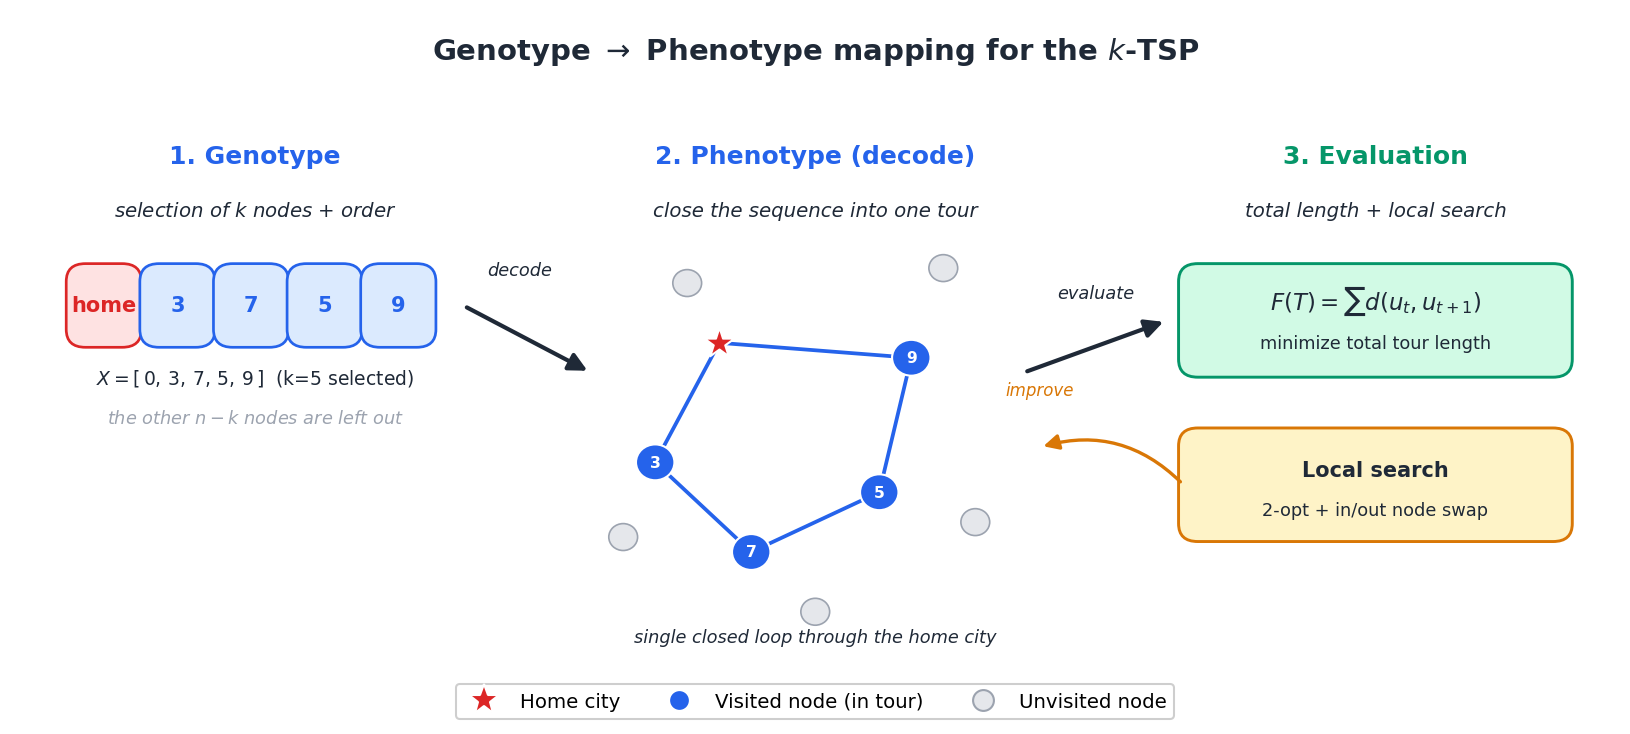
\includegraphics[width=0.7\textwidth]{Genotipo-Fenotipo.png}
\caption{Genotype--phenotype relationship of the tour-based encoding: the
selected subset and its ordering (genotype) map to a single closed loop through
the depot over the $k$ chosen nodes (phenotype).}
\label{fig:genotipo}
\end{figure}

\section{Solution Techniques}\label{sec:methods}
All methods share a common core of vectorized primitives --- \textbf{2-opt} over
the cycle, an \textbf{in/out exchange} that replaces a selected node by an
unselected one, and \textbf{cheapest insertion} --- so they differ only in how
they build and explore solutions, which makes the comparison fair. Ten techniques
are implemented and compared; LKH-3 is the source of the reference values and is
not among the methods run here.

\begin{description}[leftmargin=*,style=nextline]
  \item[Greedy (cheapest insertion).] Builds the tour from the depot by
  repeatedly inserting the node with the smallest marginal insertion cost until
  $k$ nodes are reached, then refines with 2-opt; several deterministic restarts
  keep the best tour~\cite{croes1958,rosenkrantz1977,gutin2002greedy}.
  \item[GRASP / multi-start.] A randomized greedy construction followed by local
  search (2-opt $+$ in/out exchange); the best tour over many restarts within a
  time budget is retained~\cite{feo1995grasp}.
  \item[Genetic Algorithm (GA).] An individual encodes the selected subset and
  its order; tournament selection, a subset-aware crossover, swap/in--out
  mutation, elitism and 2-opt refinement explore both the selection and the
  ordering spaces~\cite{holland1975adaptation,potvin1996}.
  \item[Nearest Neighbor (NN).] Starting from the depot, the tour is extended to
  the nearest not-yet-visited node until $k$ nodes are selected, then refined by
  local search; deterministic~\cite{rosenkrantz1977,johnson1997}.
  \item[Nearest / Farthest Insertion (NI, FI).] Insertion heuristics that place
  the incoming node at its cheapest position; NI inserts the node closest to the
  current tour, FI the farthest~\cite{rosenkrantz1977,bentley1992}.
  \item[Random Insertion (RI).] A stochastic multi-start insertion in which the
  next node is chosen uniformly at random; local search improves each
  construction~\cite{rosenkrantz1977,laporte1992}.
  \item[Simulated Annealing (SA).] A single-solution metaheuristic that accepts a
  candidate move with cost change $\Delta$ if $\Delta<0$ and otherwise with the
  Metropolis probability $\exp(-\Delta/T)$, cooling $T$
  geometrically~\cite{kirkpatrick1983,cerny1985}.
  \item[Tabu Search (TS).] A memory-based local search that, at each iteration,
  applies the best non-tabu move in the 2-opt and in/out neighbourhoods (even if
  it worsens the tour), forbids recently used moves for a fixed \emph{tenure}, and
  overrides the prohibition when a move yields a new global best (aspiration
  criterion)~\cite{glover1986,gloverlaguna1997,knox1994}.
  \item[DCIH (proposed).] The proposed \emph{deterministic} heuristic
  (Algorithm~\ref{alg:dcih}): it selects the $k$ nodes and their order by minimum
  marginal insertion cost, breaking ties by node index, and refines with 2-opt and
  an in/out exchange, so it returns exactly the same tour on every run.
\end{description}

\begin{algorithm}[t]
\small
\DontPrintSemicolon
\SetKwInput{KwIn}{Input}\SetKwInput{KwOut}{Output}
\caption{DCIH — Deterministic Cheapest-Insertion Heuristic for the $k$-TSP}
\label{alg:dcih}
\KwIn{nodes $V$, depot $0$, count $k$, distances $d$, optional window $w$}
\KwOut{tour $T$ over exactly $k$ nodes minimizing total length}
$P \leftarrow V\setminus\{0\}$\;
\If{$w>0$ \textbf{and} $w<|P|$}{$P \leftarrow$ the $w$ nodes nearest to $0$}
$s \leftarrow \arg\min_{v\in P}\,(d(0,v),v)$ \tcp*{tie-break by node index}
$T \leftarrow [\,0,\,s\,]$;\quad $P\leftarrow P\setminus\{s\}$\;
\While{$|T|<k$ \textbf{and} $P\neq\varnothing$}{
  select $v\in P$ and a position minimizing the marginal insertion cost
  $\Delta=d(a,v)+d(v,b)-d(a,b)$ over adjacent pairs $(a,b)$ of $T$ (ties by index)\;
  insert $v$ at its best position; $P\leftarrow P\setminus\{v\}$\;
}
$T \leftarrow \textbf{TwoOptCycle}(T,d)$\;
\Repeat{no improvement}{
  $T \leftarrow \textbf{SwapInOut}(T,d)$;\quad $T \leftarrow \textbf{TwoOptCycle}(T,d)$\;
}
\Return{$T$}\;
\end{algorithm}

\section{Benchmarks and Evaluation}
Experiments use 38 standard TSPLIB instances and follow the $k$-TSP benchmark of
Pandiri \& Singh~\cite{pandiri2020}, which defines three values of $k$ per
instance: \textbf{Q1} ($k=\lfloor n/4\rfloor$), \textbf{Q2} ($k=\lfloor n/2\rfloor$)
and \textbf{Q3} ($k=\lfloor 3n/4\rfloor$). Each result is compared against the
best-known value (BKS) obtained by LKH-3~\cite{Helsgaun} for the corresponding
quartile, and the relative GAP is computed as
$\mathrm{GAP}\%=100\,(\text{length}-\text{BKS})/\text{BKS}$.

Because end-of-run results alone can hide which method is preferable under a given
budget, the comparison is complemented with the \emph{anytime} benchmarking
procedure of Weise \textit{et~al.}~\cite{weise2014benchmarking}. Wall-clock time is
replaced by a \emph{machine-independent} measure --- the number of \emph{distance
evaluations} (DE), i.e.\ accesses to the distance matrix. Every run emits log
points $(\mathrm{DE},\text{length})$ each time it improves its incumbent, and
quality is the normalized error $F=\text{length}/\text{BKS}-1$. To aggregate
across instances of different size, the DE axis is scaled by $n^2$. Each
stochastic method (Greedy, GRASP, GA, RI, SA, TS) is run $10$ times per instance
and quartile; the deterministic methods (NN, NI, FI, DCIH) are run once. All
methods share a budget of $15\,n^2$ distance evaluations.

\section{Results}
Table~\ref{tab:resumen_gap} summarizes the average relative GAP per method and
quartile. Tables~\ref{tab:resultados_Q1}--\ref{tab:resultados_Q3} report the
per-instance tour lengths for Q1, Q2 and Q3; values in bold match the LKH-3
best-known value.

\begin{table}[htbp]
\centering
\caption{Average relative GAP (\%) vs the LKH-3 BKS, per method and quartile. Lower is better. Q1: $k=\lfloor n/4\rfloor$, Q2: $k=\lfloor n/2\rfloor$, Q3: $k=\lfloor 3n/4\rfloor$. Computed over 38 TSPLIB instances.}
\label{tab:resumen_gap}
\begin{tabular}{|l|c|c|c|}
\hline
\textbf{Method} & \textbf{Q1 GAP\%} & \textbf{Q2 GAP\%} & \textbf{Q3 GAP\%} \\
\hline
Greedy & 7.57 & 15.26 & 14.95 \\
GRASP & 18.03 & 19.57 & 17.39 \\
GA & 29.74 & 22.50 & 15.60 \\
NN & 22.38 & 20.04 & 15.56 \\
NI & 20.47 & 21.74 & 21.66 \\
FI & 98.23 & 55.67 & 31.63 \\
RI & 48.74 & 28.18 & 16.11 \\
SA & 15.72 & 17.81 & 17.89 \\
TS & 9.36 & 13.63 & 14.48 \\
\textbf{DCIH} & 19.83 & 23.19 & 20.36 \\
\hline
\end{tabular}
\end{table}


Across the 38 instances, the greedy cheapest-insertion baseline and Tabu Search
attain the lowest average GAP overall ($\approx 12.6\%$ and $\approx 12.5\%$),
with Tabu Search the best of the metaheuristics; Simulated Annealing follows,
ahead of GRASP and Nearest Neighbor. The genetic algorithm has a higher average
GAP but is the most frequent per-instance winner (together with Greedy) and
closes the gap for large $k$ (Q3). Among the construction heuristics, Farthest
Insertion is clearly the weakest for the $k$-TSP: repeatedly inserting the node
\emph{farthest} from the tour conflicts with the node-selection objective, which
rewards choosing nodes that are cheap to include. DCIH remains a deterministic,
reproducible alternative of quality comparable to GRASP and the insertion
heuristics.

\begin{table*}[htbp]
\centering
\caption{Results for the $k$-TSP, quartile Q1 ($k\approx n/4$). Total tour length per method; the LKH-3 column is the best-known value (BKS). Values in \textbf{bold} match the LKH-3 value.}
\label{tab:resultados_Q1}
{\scriptsize\setlength{\tabcolsep}{2.5pt}\renewcommand{\arraystretch}{0.95}%
\resizebox{\textwidth}{!}{%
\begin{tabular}{|l|c|c|c|c|c|c|c|c|c|c|c|c|c|}
\hline
\textbf{Instance} & \textbf{$n$} & \textbf{$k$} & \textbf{Grd} & \textbf{GRA} & \textbf{GA} & \textbf{NN} & \textbf{NI} & \textbf{FI} & \textbf{RI} & \textbf{SA} & \textbf{TS} & \textbf{DCIH} & \textbf{LKH-3} \\
\hline
att48 & 48 & 12 & \textbf{1925} & 2290 & \textbf{1925} & 2241 & 2304 & 3314 & \textbf{1925} & 2241 & \textbf{1925} & 2363 & 1925 \\
eil51 & 51 & 12 & 83 & 90 & \textbf{82} & 91 & 88 & 96 & \textbf{82} & 88 & 84 & 83 & 82 \\
berlin52 & 52 & 13 & \textbf{679} & 735 & \textbf{679} & 735 & 735 & 1967 & \textbf{679} & 735 & \textbf{679} & 735 & 679 \\
st70 & 70 & 17 & \textbf{120} & \textbf{120} & 153 & 127 & 166 & 213 & 162 & 166 & \textbf{120} & \textbf{120} & 120 \\
eil76 & 76 & 19 & 103 & 119 & \textbf{102} & 145 & 132 & 151 & 106 & 123 & 105 & 129 & 102 \\
pr76 & 76 & 19 & \textbf{23450} & 28379 & \textbf{23450} & 32848 & 35264 & 51947 & 24901 & 25826 & 23864 & 28089 & 23450 \\
kroA100 & 100 & 25 & 5236 & 5788 & 5040 & 5950 & 5446 & 8883 & 6212 & 5395 & 5397 & 5885 & 4931 \\
kroB100 & 100 & 25 & 4353 & 4483 & 5002 & 6538 & 4850 & 7315 & 6156 & 4850 & 4605 & 4676 & 4305 \\
kroC100 & 100 & 25 & 5026 & 5838 & 4968 & 5995 & 6506 & 6753 & 6277 & 6271 & 5768 & 6577 & 4964 \\
kroD100 & 100 & 25 & 4978 & 5062 & 5369 & 5716 & 5926 & 8488 & 5872 & 4960 & \textbf{4762} & 5449 & 4762 \\
kroE100 & 100 & 25 & 3999 & 4816 & 5249 & 4762 & 4616 & 8212 & 5402 & 4175 & 3919 & 4569 & 3905 \\
eil101 & 101 & 25 & 113 & 144 & 110 & 151 & 142 & 163 & 129 & 143 & 112 & 154 & 107 \\
lin105 & 105 & 26 & \textbf{2606} & \textbf{2606} & 3648 & \textbf{2606} & 2779 & 6644 & 3918 & 2767 & \textbf{2606} & 2881 & 2606 \\
pr107 & 107 & 26 & \textbf{8443} & 8615 & 9552 & 9028 & 8957 & 25748 & 14283 & 8666 & 8449 & 8957 & 8443 \\
pr124 & 124 & 31 & 14675 & 15091 & 15918 & 16486 & 15562 & 31720 & 23217 & 15601 & 14596 & 15618 & 14325 \\
bier127 & 127 & 31 & 10881 & 11413 & \textbf{10619} & 17271 & 11572 & 27032 & 15359 & 11778 & 10831 & 11994 & 10619 \\
ch130 & 130 & 32 & 1296 & 1367 & 1392 & 1492 & 1372 & 1841 & 1549 & 1372 & 1165 & 1373 & 1130 \\
pr136 & 136 & 34 & 22436 & 23621 & 26423 & 25211 & 24235 & 34154 & 28046 & 24235 & 23522 & 24235 & 21116 \\
gr137 & 137 & 34 & 17886 & 17702 & 20518 & 23337 & 18339 & 30790 & 22364 & 18122 & 17629 & 18496 & 17399 \\
ch150 & 150 & 37 & 1324 & 1439 & 1630 & 1420 & 1451 & 2034 & 1841 & 1330 & \textbf{1276} & 1369 & 1276 \\
kroA150 & 150 & 37 & 6497 & 6856 & 6448 & 6928 & 8173 & 9668 & 8044 & 7256 & 6832 & 7286 & 5690 \\
kroB150 & 150 & 37 & 6714 & 7089 & 6684 & 6741 & 7621 & 9075 & 7993 & 6775 & 6674 & 7802 & 5812 \\
rat195 & 195 & 48 & 587 & 590 & 670 & 590 & 607 & 762 & 713 & 607 & 607 & 624 & 554 \\
kroA200 & 200 & 50 & 7094 & 7250 & 7852 & 7994 & 8050 & 11103 & 9272 & 7478 & 7584 & 7998 & 6154 \\
kroB200 & 200 & 50 & 7394 & 7115 & 7621 & 8298 & 8523 & 11471 & 9563 & 8318 & 6493 & 7979 & 6016 \\
ts225 & 225 & 56 & 34770 & 31860 & 37708 & 30000 & 29828 & 53793 & 45975 & 29739 & 29828 & 35943 & 28828 \\
tsp225 & 225 & 56 & 1028 & 1135 & 1135 & 1189 & 1159 & 1421 & 1231 & 1141 & 1159 & 1062 & 913 \\
pr226 & 226 & 56 & 24743 & 25978 & 34810 & 24594 & 24853 & 40399 & 38722 & 24864 & 24416 & 25781 & 20033 \\
gr229 & 229 & 57 & 19413 & 25551 & 23327 & 29181 & 20749 & 53777 & 31147 & 20749 & 19747 & 20650 & 18555 \\
gil262 & 262 & 65 & 643 & 649 & 687 & 735 & 735 & 863 & 751 & 705 & 735 & 792 & 541 \\
pr264 & 264 & 66 & 9472 & 12077 & 21349 & 9616 & 9939 & 25363 & 24032 & 9824 & 9918 & 9520 & 9232 \\
a280 & 280 & 70 & 671 & 738 & 833 & 700 & 815 & 966 & 879 & 727 & 743 & 702 & 649 \\
pr299 & 299 & 74 & 12858 & 13401 & 14755 & 13448 & 13685 & 19861 & 17025 & 13598 & 12613 & 14709 & 11077 \\
lin318 & 318 & 79 & 9437 & 9915 & 11712 & 9851 & 10221 & 17277 & 13311 & 10046 & 9507 & 10753 & 8544 \\
rd400 & 400 & 100 & 3872 & 3929 & 4358 & 3721 & 4089 & 5667 & 4501 & 4024 & 4089 & 3897 & 3091 \\
fl417 & 417 & 104 & 1867 & 2483 & 5987 & 2160 & 2129 & 8097 & 7001 & 2122 & 2129 & 2129 & 1831 \\
pr439 & 439 & 109 & 22564 & 31849 & 30691 & 22386 & 22519 & 51649 & 33772 & 22572 & 22519 & 29389 & 19751 \\
pcb442 & 442 & 110 & 11369 & 14467 & 15023 & 11597 & 12179 & 17803 & 15838 & 11277 & 12179 & 13633 & 10932 \\
\hline
\end{tabular}}}
\end{table*}

\begin{table*}[htbp]
\centering
\caption{Results for the $k$-TSP, quartile Q2 ($k\approx n/2$). Total tour length per method; the LKH-3 column is the best-known value (BKS). Values in \textbf{bold} match the LKH-3 value.}
\label{tab:resultados_Q2}
{\scriptsize\setlength{\tabcolsep}{2.5pt}\renewcommand{\arraystretch}{0.95}%
\resizebox{\textwidth}{!}{%
\begin{tabular}{|l|c|c|c|c|c|c|c|c|c|c|c|c|c|}
\hline
\textbf{Instance} & \textbf{$n$} & \textbf{$k$} & \textbf{Grd} & \textbf{GRA} & \textbf{GA} & \textbf{NN} & \textbf{NI} & \textbf{FI} & \textbf{RI} & \textbf{SA} & \textbf{TS} & \textbf{DCIH} & \textbf{LKH-3} \\
\hline
att48 & 48 & 24 & 3814 & 4197 & 3797 & 3924 & 3943 & 6477 & 4614 & 3744 & \textbf{3603} & 4943 & 3603 \\
eil51 & 51 & 25 & 188 & 189 & 181 & 197 & 199 & 239 & 192 & 193 & \textbf{175} & 198 & 175 \\
berlin52 & 52 & 26 & 1995 & 2019 & \textbf{1874} & \textbf{1874} & 2061 & 5291 & 1952 & \textbf{1874} & \textbf{1874} & 2269 & 1874 \\
st70 & 70 & 35 & 293 & 284 & 277 & 323 & 313 & 384 & 307 & 303 & 287 & 302 & 260 \\
eil76 & 76 & 38 & 231 & 260 & 220 & 233 & 249 & 273 & 238 & 240 & 231 & 249 & 213 \\
pr76 & 76 & 38 & 45066 & 50069 & 42800 & 47591 & 62194 & 65376 & 49087 & 49622 & 45459 & 51378 & 41248 \\
kroA100 & 100 & 50 & 10650 & 10528 & 9895 & 12246 & 12164 & 12938 & 11377 & 11202 & 9610 & 12532 & 9184 \\
kroB100 & 100 & 50 & 9842 & 9278 & 10952 & 12750 & 10628 & 12697 & 11281 & 10325 & 9640 & 11557 & 9096 \\
kroC100 & 100 & 50 & 11220 & 10458 & 10348 & 11018 & 12853 & 12522 & 10839 & 12710 & 10577 & 12916 & 9457 \\
kroD100 & 100 & 50 & 10233 & 10769 & 9483 & 11145 & 11593 & 12706 & 10659 & 10259 & 9349 & 11438 & 8719 \\
kroE100 & 100 & 50 & 9878 & 9886 & 10995 & 9926 & 10916 & 12561 & 11126 & 10559 & 10466 & 11043 & 9097 \\
eil101 & 101 & 50 & 263 & 295 & 245 & 331 & 269 & 338 & 258 & 259 & 246 & 276 & 227 \\
lin105 & 105 & 52 & 5952 & 6677 & 5960 & 6171 & 6612 & 9784 & 7552 & 6442 & 6033 & 6066 & 5848 \\
pr107 & 107 & 53 & 18211 & 18383 & 30949 & 18650 & 18328 & 32890 & 30942 & 18154 & 18191 & 18328 & 18028 \\
pr124 & 124 & 62 & 27487 & 32502 & 31630 & 25386 & 27448 & 43178 & 37192 & 27448 & 27448 & 27487 & 22998 \\
bier127 & 127 & 63 & 27882 & 28568 & 34757 & 29733 & 31153 & 54960 & 36698 & 30050 & 27583 & 28900 & 25761 \\
ch130 & 130 & 65 & 2972 & 2923 & 2773 & 2781 & 3009 & 3424 & 3120 & 2979 & 2781 & 3145 & 2408 \\
pr136 & 136 & 68 & 47633 & 52280 & 50367 & 50325 & 50223 & 59154 & 50143 & 50223 & 50223 & 48682 & 46414 \\
gr137 & 137 & 68 & 32687 & 34337 & 35937 & 40207 & 34435 & 39862 & 36234 & 34042 & 30794 & 33083 & 29231 \\
ch150 & 150 & 75 & 3271 & 3386 & 3469 & 3405 & 3215 & 3773 & 3441 & 3215 & 2972 & 3483 & 2760 \\
kroA150 & 150 & 75 & 14593 & 13927 & 13024 & 15031 & 14671 & 17295 & 14255 & 14608 & 13569 & 15061 & 11496 \\
kroB150 & 150 & 75 & 13604 & 14125 & 12803 & 13376 & 14511 & 14915 & 13165 & 13151 & 12747 & 15202 & 11357 \\
rat195 & 195 & 97 & 1201 & 1222 & 1281 & 1163 & 1246 & 1445 & 1285 & 1238 & 1246 & 1230 & 1100 \\
kroA200 & 200 & 100 & 15560 & 14408 & 15905 & 14246 & 15896 & 17895 & 15478 & 15629 & 15896 & 16045 & 12372 \\
kroB200 & 200 & 100 & 15053 & 14675 & 15226 & 17343 & 16089 & 18482 & 15411 & 14877 & 14101 & 16237 & 12338 \\
ts225 & 225 & 112 & 71402 & 66992 & 71441 & 64093 & 70167 & 83583 & 69459 & 70614 & 70167 & 69307 & 56828 \\
tsp225 & 225 & 112 & 2094 & 2077 & 2031 & 2022 & 2175 & 2334 & 2096 & 2159 & 2175 & 2086 & 1708 \\
pr226 & 226 & 113 & 55362 & 48157 & 46348 & 56774 & 55560 & 60717 & 48782 & 55560 & 49771 & 50141 & 36720 \\
gr229 & 229 & 114 & 44764 & 48341 & 57572 & 57075 & 44489 & 78396 & 62419 & 44452 & 44489 & 49566 & 39618 \\
gil262 & 262 & 131 & 1265 & 1317 & 1244 & 1185 & 1362 & 1455 & 1276 & 1341 & 1362 & 1377 & 993 \\
pr264 & 264 & 132 & 23188 & 23194 & 31851 & 22934 & 23984 & 33995 & 32338 & 23547 & 23984 & 23234 & 22644 \\
a280 & 280 & 140 & 1298 & 1425 & 1494 & 1417 & 1453 & 1703 & 1555 & 1432 & 1453 & 1382 & 1231 \\
pr299 & 299 & 149 & 26280 & 26457 & 27744 & 26624 & 25231 & 30532 & 27358 & 25251 & 25231 & 27199 & 22390 \\
lin318 & 318 & 159 & 20313 & 21127 & 21532 & 21405 & 21718 & 25343 & 21910 & 21402 & 21718 & 20949 & 15916 \\
rd400 & 400 & 200 & 7895 & 8077 & 8627 & 7641 & 8332 & 8964 & 8240 & 8253 & 8332 & 7990 & 6350 \\
fl417 & 417 & 208 & 6059 & 6485 & 8160 & 6235 & 6018 & 9171 & 8002 & 5954 & 6018 & 6162 & 5436 \\
pr439 & 439 & 219 & 41861 & 58306 & 59080 & 44124 & 42048 & 74565 & 57457 & 41917 & 42048 & 54542 & 35404 \\
pcb442 & 442 & 221 & 24374 & 29122 & 29106 & 24841 & 25403 & 30999 & 29123 & 24063 & 25403 & 27608 & 22537 \\
\hline
\end{tabular}}}
\end{table*}

\begin{table*}[htbp]
\centering
\caption{Results for the $k$-TSP, quartile Q3 ($k\approx 3n/4$). Total tour length per method; the LKH-3 column is the best-known value (BKS). Values in \textbf{bold} match the LKH-3 value.}
\label{tab:resultados_Q3}
{\scriptsize\setlength{\tabcolsep}{2.5pt}\renewcommand{\arraystretch}{0.95}%
\resizebox{\textwidth}{!}{%
\begin{tabular}{|l|c|c|c|c|c|c|c|c|c|c|c|c|c|}
\hline
\textbf{Instance} & \textbf{$n$} & \textbf{$k$} & \textbf{Grd} & \textbf{GRA} & \textbf{GA} & \textbf{NN} & \textbf{NI} & \textbf{FI} & \textbf{RI} & \textbf{SA} & \textbf{TS} & \textbf{DCIH} & \textbf{LKH-3} \\
\hline
att48 & 48 & 36 & 6710 & 6699 & 7049 & 7045 & 7036 & 8785 & 7435 & 6691 & 6581 & 6863 & 6563 \\
eil51 & 51 & 38 & 297 & 300 & 295 & 302 & 326 & 314 & 296 & 294 & 302 & 316 & 287 \\
berlin52 & 52 & 39 & 4349 & 4250 & 4340 & 4708 & 5162 & 5943 & 4561 & 4631 & 4490 & 4627 & 4174 \\
st70 & 70 & 52 & 447 & 454 & 482 & 485 & 511 & 506 & 466 & 485 & 433 & 486 & 428 \\
eil76 & 76 & 57 & 358 & 388 & 365 & 353 & 405 & 413 & 375 & 372 & 352 & 376 & 335 \\
pr76 & 76 & 57 & 65621 & 72347 & 76427 & 70284 & 79931 & 86418 & 74391 & 74776 & 67540 & 70861 & 64142 \\
kroA100 & 100 & 75 & 16900 & 15894 & 15459 & 15658 & 17234 & 17000 & 15572 & 16907 & 15489 & 18142 & 14379 \\
kroB100 & 100 & 75 & 16916 & 16401 & 16233 & 17576 & 16488 & 18461 & 16019 & 16299 & 15614 & 18413 & 14680 \\
kroC100 & 100 & 75 & 17204 & 16279 & 15129 & 14815 & 18783 & 17126 & 15221 & 16418 & 14358 & 18390 & 13892 \\
kroD100 & 100 & 75 & 15438 & 15753 & 14938 & 16450 & 18327 & 17374 & 15972 & 16838 & 15021 & 17539 & 14058 \\
kroE100 & 100 & 75 & 16748 & 17097 & 15494 & 17020 & 18255 & 17367 & 16210 & 17988 & 16098 & 17372 & 14622 \\
eil101 & 101 & 75 & 433 & 439 & 422 & 446 & 442 & 482 & 421 & 449 & 414 & 458 & 386 \\
lin105 & 105 & 78 & 9274 & 10173 & 10175 & 9566 & 10056 & 12496 & 10649 & 9482 & 9252 & 9388 & 8983 \\
pr107 & 107 & 80 & 38179 & 37644 & 37944 & 37688 & 40687 & 38940 & 37700 & 39058 & 38406 & 38780 & 36292 \\
pr124 & 124 & 93 & 40484 & 45096 & 44968 & 42339 & 40385 & 59259 & 44605 & 40385 & 40385 & 40506 & 39008 \\
bier127 & 127 & 95 & 51722 & 51931 & 58088 & 65610 & 58529 & 84422 & 62716 & 54586 & 52983 & 53130 & 49680 \\
ch130 & 130 & 97 & 4446 & 4409 & 4428 & 4520 & 4541 & 5025 & 4376 & 4518 & 4295 & 4712 & 3876 \\
pr136 & 136 & 102 & 75924 & 74084 & 71668 & 81225 & 79538 & 82300 & 72066 & 78431 & 73028 & 75924 & 67910 \\
gr137 & 137 & 102 & 51429 & 50490 & 47941 & 46744 & 54376 & 53533 & 48175 & 52598 & 47710 & 51852 & 43670 \\
ch150 & 150 & 112 & 5098 & 5062 & 4934 & 4910 & 5185 & 5471 & 4951 & 5185 & 5185 & 5171 & 4366 \\
kroA150 & 150 & 112 & 20696 & 20815 & 19639 & 21619 & 21097 & 22727 & 19837 & 20877 & 21097 & 21792 & 17395 \\
kroB150 & 150 & 112 & 20092 & 20330 & 19016 & 18239 & 21481 & 20530 & 18761 & 20800 & 18820 & 21431 & 16879 \\
rat195 & 195 & 146 & 1812 & 1880 & 1911 & 1757 & 1877 & 1951 & 1916 & 1853 & 1877 & 1821 & 1667 \\
kroA200 & 200 & 150 & 23738 & 23281 & 23339 & 22004 & 25097 & 24322 & 22445 & 24608 & 21407 & 24098 & 19211 \\
kroB200 & 200 & 150 & 23709 & 22672 & 22118 & 24041 & 24364 & 23720 & 22532 & 24023 & 24364 & 24702 & 18898 \\
ts225 & 225 & 168 & 100138 & 102165 & 100233 & 98141 & 105659 & 104831 & 97765 & 105134 & 105659 & 104329 & 85656 \\
tsp225 & 225 & 168 & 3096 & 3066 & 3092 & 2978 & 3365 & 3332 & 3015 & 3192 & 3365 & 3139 & 2624 \\
pr226 & 226 & 169 & 76096 & 67041 & 55617 & 71619 & 73540 & 79205 & 58094 & 72995 & 73540 & 78642 & 47142 \\
gr229 & 229 & 171 & 71551 & 79083 & 95317 & 79477 & 73693 & 116715 & 90428 & 73373 & 73693 & 74369 & 64457 \\
gil262 & 262 & 196 & 1815 & 1903 & 1869 & 1849 & 1938 & 1984 & 1842 & 1929 & 1938 & 1930 & 1551 \\
pr264 & 264 & 198 & 41226 & 40419 & 40415 & 37969 & 41812 & 42945 & 40687 & 41349 & 41812 & 41954 & 34346 \\
a280 & 280 & 210 & 2059 & 2216 & 2127 & 2057 & 2174 & 2345 & 2155 & 2128 & 2174 & 2190 & 1845 \\
pr299 & 299 & 224 & 38539 & 40335 & 38679 & 38391 & 39357 & 41816 & 38249 & 39314 & 39357 & 40393 & 32738 \\
lin318 & 318 & 238 & 31760 & 32456 & 33651 & 32139 & 33120 & 36147 & 32584 & 32647 & 33120 & 32784 & 25303 \\
rd400 & 400 & 300 & 11910 & 12195 & 12139 & 11639 & 12341 & 12274 & 11979 & 12197 & 12341 & 12030 & 9972 \\
fl417 & 417 & 312 & 10539 & 11375 & 9355 & 10143 & 10820 & 11559 & 9650 & 10805 & 10820 & 11403 & 7930 \\
pr439 & 439 & 329 & 67177 & 84057 & 90201 & 74522 & 68148 & 99252 & 87209 & 67964 & 68148 & 76775 & 58006 \\
pcb442 & 442 & 331 & 38114 & 43408 & 40379 & 36174 & 40401 & 44072 & 42149 & 38507 & 40401 & 40135 & 34358 \\
\hline
\end{tabular}}}
\end{table*}


\section{Anytime Evaluation}
From the logged trajectories we build three standard views. The
\textbf{progress curves} (Figure~\ref{fig:progress}) show the median best-so-far
error $F$ versus the scaled DE; all methods are drawn over a common budget, so a
method that converges early appears as a flat line. The \textbf{ECDF}
(Figure~\ref{fig:ecdf}) shows the fraction of runs that reach the target error
$F_t=20\%$ as a function of the scaled DE, and the \textbf{ERT}
(Figure~\ref{fig:ert}) reports the estimated running time to reach each target
error. Aggregating four criteria (final $F$, area under the progress and ECDF
curves, and ERT at $20\%$) by the median rank yields the global ranking of
Table~\ref{tab:anytime_ranking}.

\begin{figure}[t]
\centering
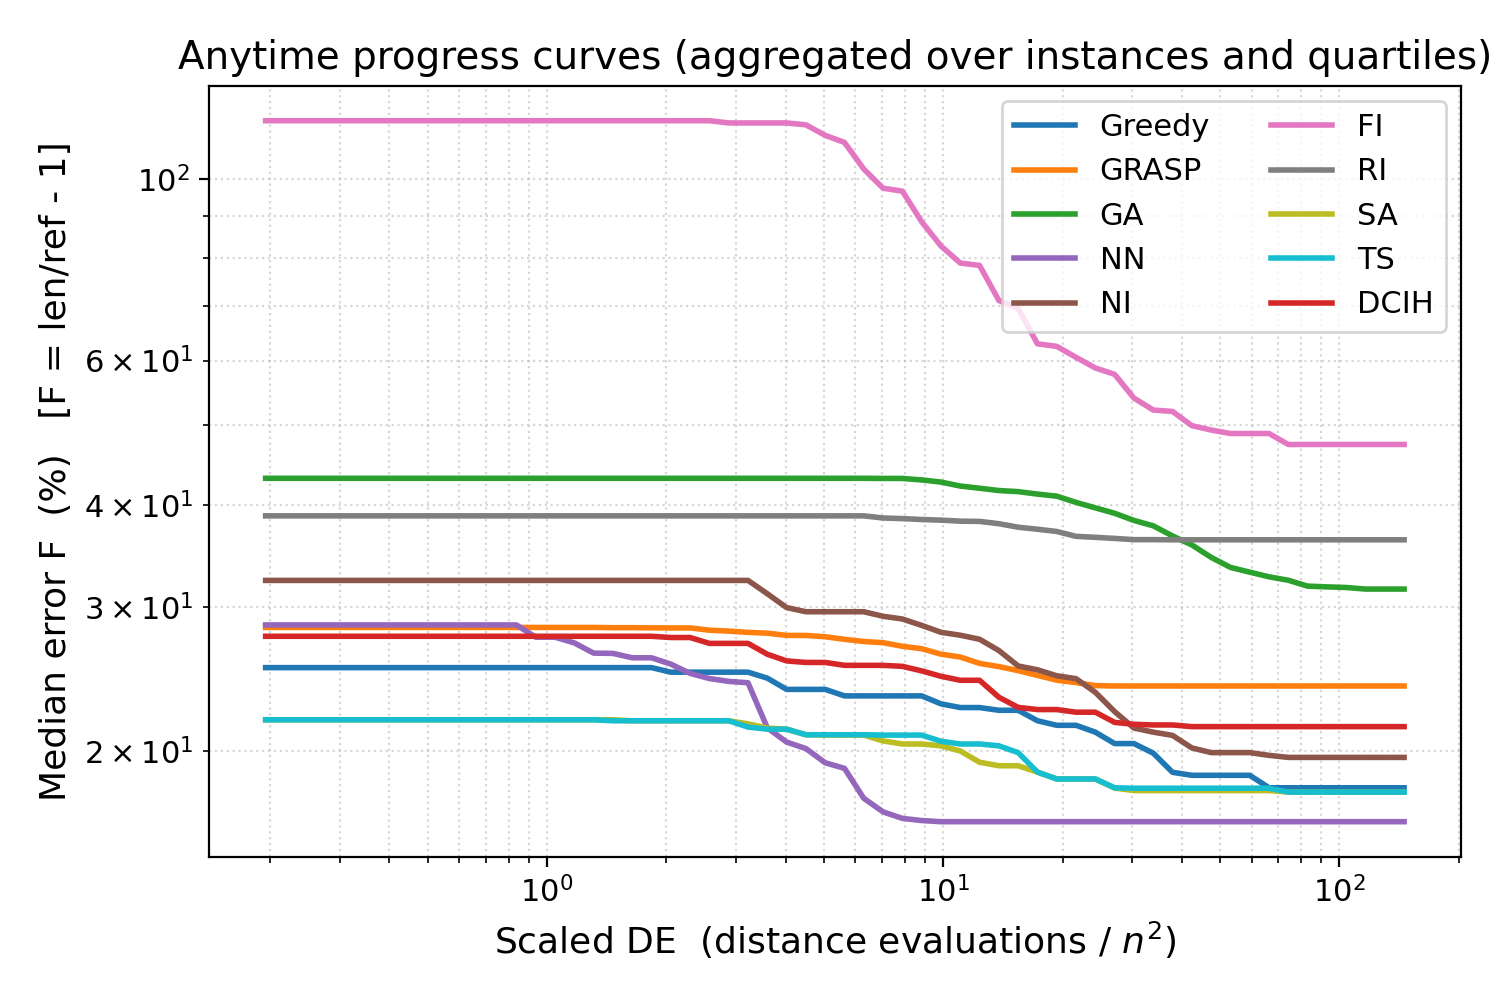
\includegraphics[width=0.9\textwidth]{01_progreso_agregado.png}
\caption{Anytime progress curves aggregated over the 38 TSPLIB instances and the
three quartiles of $k$: median error $F$ (\%) versus the machine-independent time
(distance evaluations scaled by $n^2$). Lower and earlier is better.}
\label{fig:progress}
\end{figure}

\begin{figure}[t]
\centering
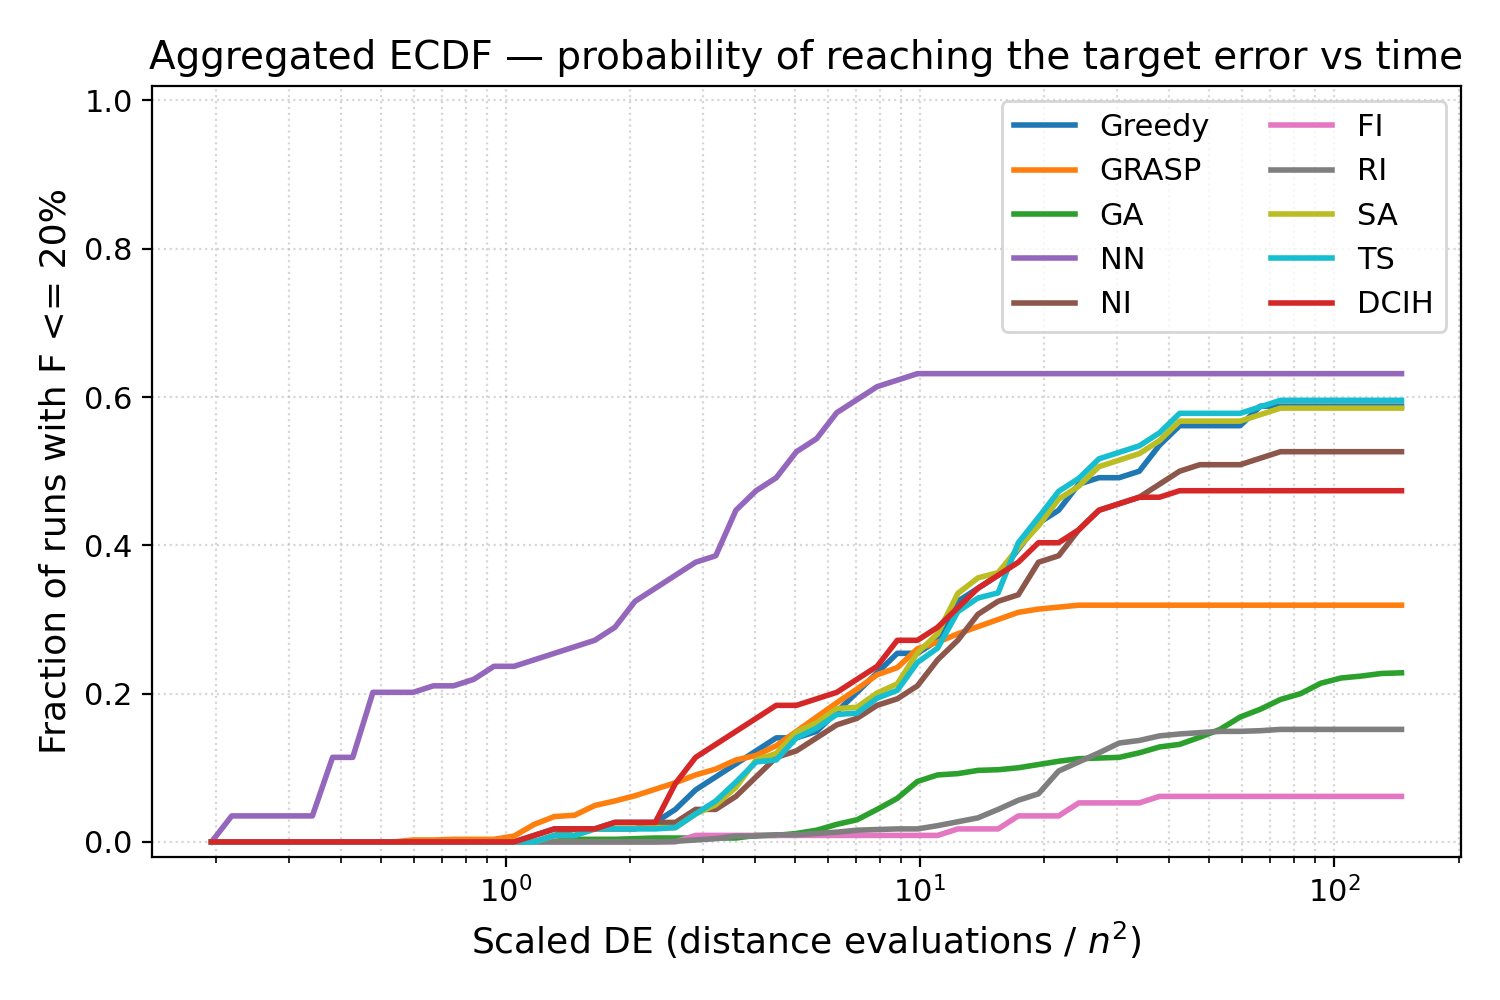
\includegraphics[width=0.9\textwidth]{02_ecdf_agregado.png}
\caption{Aggregated ECDF for the target error $F_t=20\%$: fraction of runs that
reach a tour within $20\%$ of the LKH-3 reference as a function of the scaled
distance evaluations.}
\label{fig:ecdf}
\end{figure}

\begin{figure}[t]
\centering
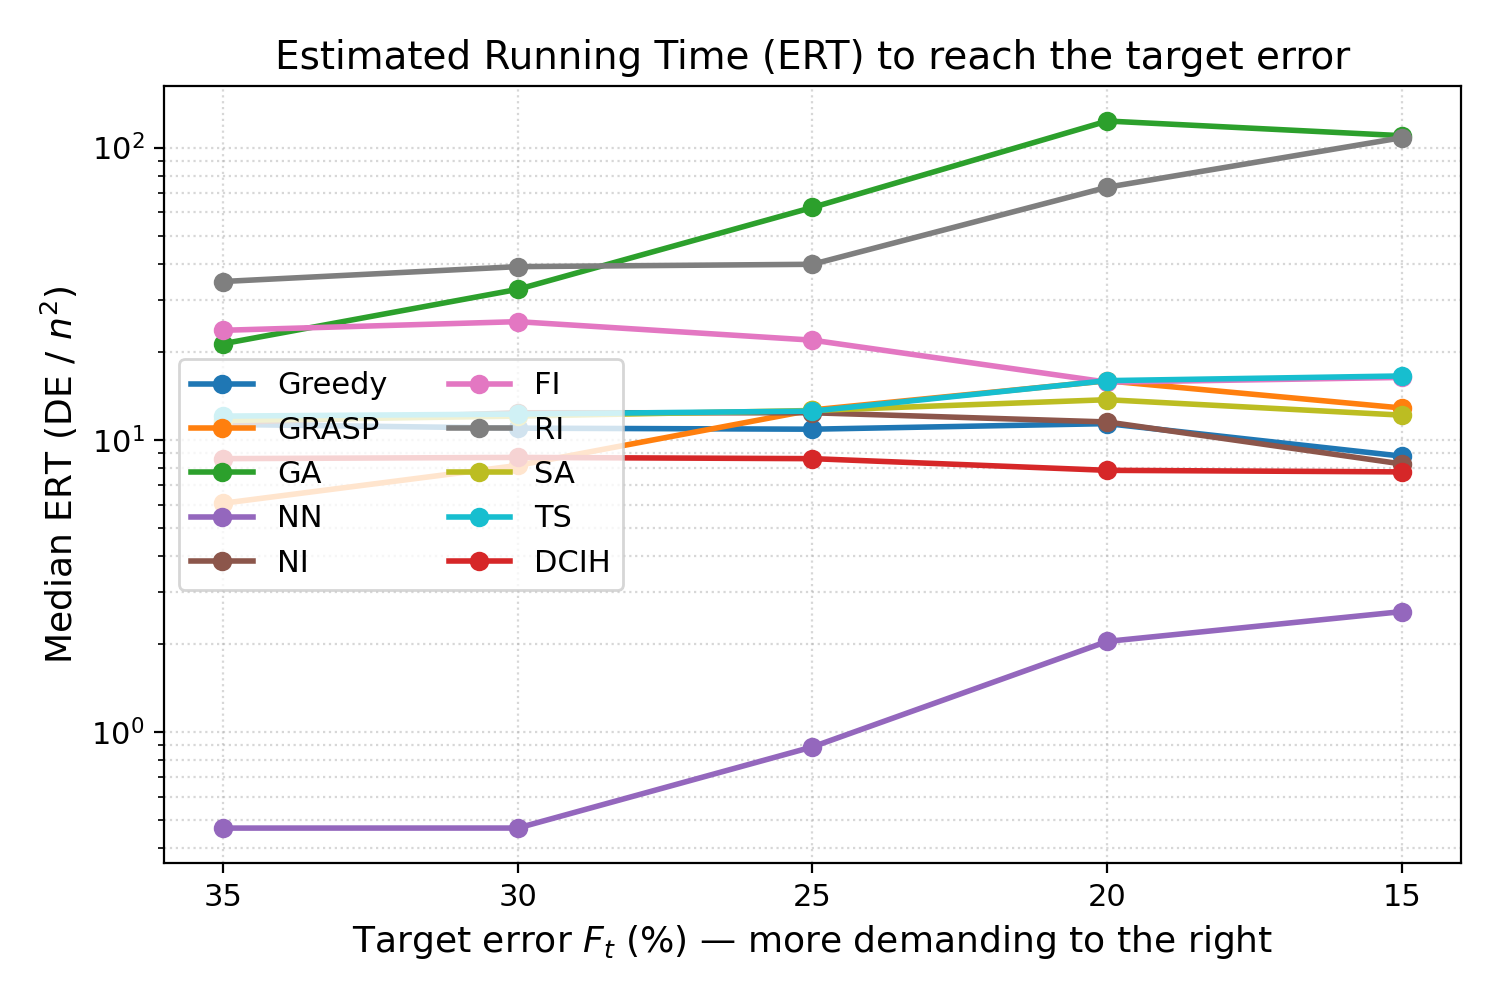
\includegraphics[width=0.9\textwidth]{03_ert_vs_meta.png}
\caption{Median ERT (scaled distance evaluations, $\mathrm{DE}/n^2$) to reach each
target error $F_t$ (from $35\%$ down to $15\%$; more demanding to the right).}
\label{fig:ert}
\end{figure}

\begin{table}[htbp]
\centering
\caption{Anytime \textbf{global ranking} (median rank, lower is better) aggregating four criteria over the 38 TSPLIB instances and the three quartiles of $k$, with the LKH-3 value as reference.}
\label{tab:anytime_ranking}
\begin{tabular}{|l|c|c|c|c|c|}
\hline
\textbf{Method} & \textbf{Final} & \textbf{AUC} & \textbf{AUC} & \textbf{ERT} & \textbf{Global} \\
                & \textbf{$F$}   & \textbf{prog.}& \textbf{ECDF}& \textbf{@20\%}& \textbf{rank} \\
\hline
\textbf{NN} & 3.0 & 9.0 & 1.0 & 1.00 & \textbf{2.00} \\
Greedy & 4.0 & 3.2 & 5.0 & 5.00 & 4.50 \\
TS & 4.0 & 2.5 & 5.0 & 5.50 & 4.50 \\
SA & 4.0 & 2.0 & 5.2 & 5.50 & 4.62 \\
\textbf{DCIH} & 5.0 & 5.0 & 5.5 & 5.50 & 5.25 \\
NI & 5.0 & 4.0 & 6.0 & 6.00 & 5.50 \\
GRASP & 6.0 & 8.0 & 6.0 & 6.00 & 6.00 \\
GA & 8.0 & 9.0 & 7.0 & 7.00 & 7.50 \\
RI & 9.0 & 6.0 & 7.5 & 7.50 & 7.50 \\
FI & 10.0 & 9.0 & 8.0 & 8.00 & 8.50 \\
\hline
\end{tabular}
\end{table}


Under a fixed machine-independent budget, Nearest Neighbor ranks first because it
reaches a good tour with far fewer distance evaluations than any other method, so
it dominates the ERT and ECDF criteria; the greedy baseline, Tabu Search and
Simulated Annealing follow, and DCIH provides a competitive \emph{deterministic}
trajectory with no variance across runs. Farthest Insertion ranks last. The
contrast between the anytime ranking (which rewards fast convergence) and the
end-of-run GAP (which rewards final quality) is exactly the kind of insight the
anytime methodology is designed to expose~\cite{weise2014benchmarking}.

\section{Analysis of the Generated Tours}
The tours produced for the $k$-TSP are single closed loops through the depot over
a selected subset of $k$ nodes. The cheapest-insertion constructive methods
(Greedy, NI, DCIH) select nodes that are cheap to insert, yielding compact loops,
whereas Farthest Insertion deliberately picks distant nodes and produces long,
sprawling tours that local search only partly repairs. Nearest Neighbor builds a
short chain greedily but can be trapped by a costly final return edge. The
population- and trajectory-based methods (GRASP, GA, RI, SA, TS) explore
alternative subsets that can shorten the tour further. After 2-opt and the in/out
exchange, crossings are removed and the selected subset stabilizes around nodes
that are cheap to include.

\clearpage

% ============================================================================
%  CHAPTER 3 — CONCLUSIONS AND FUTURE WORK
% ============================================================================
\chapter{Conclusions and Future Work}

This thesis implemented and compared ten methods for the $k$-Traveling Salesman
Problem --- a greedy cheapest-insertion heuristic, a GRASP/multi-start scheme, a
genetic algorithm, the Nearest Neighbor and the Nearest, Farthest and Random
Insertion heuristics, Simulated Annealing, Tabu Search, and the proposed
deterministic heuristic DCIH --- and evaluated them on 38 TSPLIB instances across
three values of $k$, using the best-known values obtained by LKH-3 as the quality
reference. Beyond the end-of-run comparison, the study adopted the anytime
benchmarking methodology of Weise \textit{et~al.}, reporting progress curves,
ERT, ECDF and an aggregated global ranking on a machine-independent time axis.

\section{Main Conclusions}
\begin{itemize}[leftmargin=*]
  \item The greedy cheapest-insertion baseline is the most robust method on
  average across the whole range of $k$, and \textbf{Tabu Search is the best of
  the metaheuristics}, essentially tying the baseline in average GAP.
  \item The genetic algorithm matches the baseline and becomes the most frequent
  per-instance winner only for large $k$ (Q3), consistent with its slower but
  continuing convergence observed in the progress curves.
  \item \textbf{Farthest Insertion is the weakest} method for the $k$-TSP:
  selecting the nodes farthest from the tour conflicts with the node-selection
  objective, which rewards cheap-to-include nodes.
  \item The proposed \textbf{DCIH} provides a deterministic, fully reproducible
  alternative of quality comparable to GRASP and the insertion heuristics ---
  useful whenever reproducibility matters more than winning by chance.
  \item The anytime analysis revealed a distinction that end-of-run tables hide:
  under a limited budget, the very cheap Nearest Neighbor dominates the
  \emph{speed} criteria (ERT, ECDF) even though it is only mid-ranked in final
  quality. Separating ``fast'' from ``best'' is precisely the value of the anytime
  methodology.
\end{itemize}

\section{Contributions}
The main contributions of this work are: (i)~a reproducible, openly documented
repository in which every table and figure can be regenerated with a single
command; (ii)~a uniform implementation of ten $k$-TSP methods over a shared
local-search core, enabling a fair comparison; (iii)~the proposed deterministic
DCIH heuristic; and (iv)~an anytime, machine-independent evaluation of the methods
against the LKH-3 reference.

\section{Future Work}
Several directions remain open. First, more powerful metaheuristics --- such as
ant colony optimization~\cite{dorigo1997acs}, variable neighborhood
search~\cite{mladenovic1997vns} or hybrid (memetic) schemes combining Tabu Search
with the genetic algorithm --- could narrow the gap to LKH-3, especially for large
$k$. Second, parameter tuning (tabu tenure, cooling schedule, population size) was
kept fixed for fairness and could be optimized per instance size. Third, the
node-selection component could be strengthened with dedicated selection rules
rather than relying on insertion cost alone. Finally, extending the reproducible
framework to larger TSPLIB instances and to related selective-routing problems
(Orienteering, Prize-Collecting TSP) would broaden the scope of the comparison.

\clearpage

% ============================================================================
%  BIBLIOGRAPHY (50 references)
% ============================================================================
\begin{thebibliography}{00}
\bibitem{ene2017} A. Ene, V. Nagarajan, R. Saket, 
``Approximation Algorithms for Stochastic $k$-TSP,'' 2017.

\bibitem{venkatesh2018} P. Venkatesh, G. Srivastava, A. Singh, 
``A GVNS heuristic for $k$-TSP,'' 
\textit{Procedia Computer Science}, vol. 143, pp. 189--196, 2018.

\bibitem{pandiri2020} V. Pandiri and A. Singh, 
``Two multi-start heuristics for the $k$-traveling salesman problem,'' 
\textit{OPSEARCH}, vol. 57, pp. 1164--1204, 2020.

\bibitem{blanchard2023} M. Blanchard, A. Jacquillat, P. Jaillet, 
``Probabilistic bounds on $k$-TSP,'' 
\textit{arXiv:2211.11063}, 2023.

\bibitem{Helsgaun} K. Helsgaun, 
``An effective implementation of the Lin-Kernighan traveling salesman heuristic,'' 
\textit{European Journal of Operational Research}, vol. 126, no. 1, pp. 106--130, 2000.

\bibitem{helsgaun2017lkh3} K. Helsgaun, 
``An extension of the Lin-Kernighan-Helsgaun TSP solver for constrained traveling salesman and vehicle routing problems,'' 
Technical Report, Roskilde University, Denmark, 2017.

\bibitem{vansteenwegen2011top} P. Vansteenwegen, W. Souffriau, and D. Van Oudheusden, 
``The Orienteering Problem: A survey,'' 
\textit{European Journal of Operational Research}, vol. 209, no. 1, pp. 1--10, 2011.

\bibitem{feo1995grasp} T. A. Feo and M. G. C. Resende, 
``Greedy Randomized Adaptive Search Procedures,'' 
\textit{Journal of Global Optimization}, vol. 6, no. 2, pp. 109--133, 1995.

\bibitem{holland1975adaptation} J. H. Holland, 
\textit{Adaptation in Natural and Artificial Systems}. University of Michigan Press, 1975.

\bibitem{lawler1985} E. L. Lawler, J. K. Lenstra, A. H. G. Rinnooy Kan, and D. B. Shmoys, 
``The Traveling Salesman Problem: A Guided Tour of Combinatorial Optimization,'' 
\textit{Wiley}, 1985.

\bibitem{miller1960mtz} C. E. Miller, A. W. Tucker, y R. A. Zemlin, 
``Integer programming formulation of traveling salesman problems,'' 
\textit{Journal of the ACM}, vol. 7, no. 4, pp. 326--329, 1960.

\bibitem{lin1973} S. Lin y B. W. Kernighan, 
``An effective heuristic algorithm for the traveling-salesman problem,'' 
\textit{Operations Research}, vol. 21, no. 2, pp. 498--516, 1973.

\bibitem{croes1958} G. A. Croes, 
``A method for solving traveling-salesman problems,'' 
\textit{Operations Research}, vol. 6, no. 6, pp. 791--812, 1958.

\bibitem{TSPLIB} G. Reinelt,
``TSPLIB—A traveling salesman problem library,''
\textit{ORSA Journal on Computing}, vol. 3, no. 4, pp. 376--384, 1991.
Disponible en: \url{https://comopt.ifi.uni-heidelberg.de/software/TSPLIB95/}

\bibitem{rego2011tsp} C. Rego, D. Gamboa, F. Glover, and C. Osterman,
``Traveling salesman problem heuristics: Leading methods, implementations and latest advances,''
\textit{European Journal of Operational Research}, vol. 211, no. 3, pp. 427--441, 2011.

\bibitem{brodowsky2023kopt} U. A. Brodowsky, S. Hougardy, and X. Zhong,
``The approximation ratio of the $k$-Opt heuristic for the Euclidean traveling salesman problem,''
\textit{SIAM Journal on Computing}, vol. 52, no. 4, pp. 841--864, 2023.

\bibitem{heimann2025kopt} S. Heimann, H. P. Hoang, and S. Hougardy,
``A near-complete resolution of the exponential-time complexity of $k$-opt for the traveling salesman problem,''
\textit{arXiv:2507.12304}, 2025.

\bibitem{gutin2002greedy} G. Gutin, A. Yeo, and A. Zverovich,
``Traveling salesman should not be greedy: domination analysis of greedy-type heuristics for the TSP,''
\textit{Discrete Applied Mathematics}, vol. 117, no. 1--3, pp. 81--86, 2002.

\bibitem{balas1989pctsp} E. Balas,
``The prize collecting traveling salesman problem,''
\textit{Networks}, vol. 19, no. 6, pp. 621--636, 1989.

\bibitem{bienstock1993pctsp} D. Bienstock, M. X. Goemans, D. Simchi-Levi, and D. Williamson,
``A note on the prize collecting traveling salesman problem,''
\textit{Mathematical Programming}, vol. 59, no. 1--3, pp. 413--420, 1993.

\bibitem{feillet2005profits} D. Feillet, P. Dejax, and M. Gendreau,
``Traveling salesman problems with profits,''
\textit{Transportation Science}, vol. 39, no. 2, pp. 188--205, 2005.

\bibitem{gunawan2016op} A. Gunawan, H. C. Lau, and P. Vansteenwegen,
``Orienteering problem: A survey of recent variants, solution approaches and applications,''
\textit{European Journal of Operational Research}, vol. 255, no. 2, pp. 315--332, 2016.

\bibitem{tspt3co2025} S. Hougardy and X. Zhong,
``A survey on approximability of traveling salesman problems using the TSP-T3CO definition scheme,''
\textit{Annals of Operations Research}, 2025. doi:10.1007/s10479-025-06641-5

\bibitem{drake2020hyper} J. H. Drake, A. Kheiri, E. \"Ozcan, and E. K. Burke,
``Recent advances in selection hyper-heuristics,''
\textit{European Journal of Operational Research}, vol. 285, no. 2, pp. 405--428, 2020.

\bibitem{applegate2006concorde} D. L. Applegate, R. E. Bixby, V. Chv\'atal, and W. J. Cook,
\textit{The Traveling Salesman Problem: A Computational Study}.
Princeton, NJ: Princeton University Press, 2006.

\bibitem{weise2014benchmarking} T. Weise, R. Chiong, J. L\"assig, K. Tang, S. Tsutsui, W. Chen, Z. Michalewicz, and X. Yao,
``Benchmarking optimization algorithms: An open source framework for the traveling salesman problem,''
\textit{IEEE Computational Intelligence Magazine}, vol. 9, no. 3, pp. 40--52, 2014.

\bibitem{rosenkrantz1977} D. J. Rosenkrantz, R. E. Stearns, and P. M. Lewis II,
``An analysis of several heuristics for the traveling salesman problem,''
\textit{SIAM Journal on Computing}, vol. 6, no. 3, pp. 563--581, 1977.

\bibitem{kirkpatrick1983} S. Kirkpatrick, C. D. Gelatt, and M. P. Vecchi,
``Optimization by simulated annealing,''
\textit{Science}, vol. 220, no. 4598, pp. 671--680, 1983.

\bibitem{dantzig1954} G. Dantzig, R. Fulkerson, and S. Johnson,
``Solution of a large-scale traveling-salesman problem,''
\textit{Operations Research}, vol. 2, no. 4, pp. 393--410, 1954.

\bibitem{bellman1962} R. Bellman,
``Dynamic programming treatment of the travelling salesman problem,''
\textit{Journal of the ACM}, vol. 9, no. 1, pp. 61--63, 1962.

\bibitem{heldkarp1962} M. Held and R. M. Karp,
``A dynamic programming approach to sequencing problems,''
\textit{Journal of the SIAM}, vol. 10, no. 1, pp. 196--210, 1962.

\bibitem{karp1972} R. M. Karp,
``Reducibility among combinatorial problems,''
in \textit{Complexity of Computer Computations}, R. E. Miller and J. W. Thatcher, Eds.
New York: Plenum Press, 1972, pp. 85--103.

\bibitem{lin1965} S. Lin,
``Computer solutions of the traveling salesman problem,''
\textit{Bell System Technical Journal}, vol. 44, no. 10, pp. 2245--2269, 1965.

\bibitem{christofides1976} N. Christofides,
``Worst-case analysis of a new heuristic for the travelling salesman problem,''
Graduate School of Industrial Administration, Carnegie Mellon University,
Report 388, 1976.

\bibitem{bentley1992} J. L. Bentley,
``Fast algorithms for geometric traveling salesman problems,''
\textit{ORSA Journal on Computing}, vol. 4, no. 4, pp. 387--411, 1992.

\bibitem{johnson1997} D. S. Johnson and L. A. McGeoch,
``The traveling salesman problem: A case study in local optimization,''
in \textit{Local Search in Combinatorial Optimization}, E. Aarts and J. K. Lenstra, Eds.
Chichester: Wiley, 1997, pp. 215--310.

\bibitem{laporte1992} G. Laporte,
``The traveling salesman problem: An overview of exact and approximate algorithms,''
\textit{European Journal of Operational Research}, vol. 59, no. 2, pp. 231--247, 1992.

\bibitem{arora1998} S. Arora,
``Polynomial time approximation schemes for Euclidean traveling salesman and other geometric problems,''
\textit{Journal of the ACM}, vol. 45, no. 5, pp. 753--782, 1998.

\bibitem{glover1986} F. Glover,
``Future paths for integer programming and links to artificial intelligence,''
\textit{Computers \& Operations Research}, vol. 13, no. 5, pp. 533--549, 1986.

\bibitem{cerny1985} V. \v{C}ern\'y,
``Thermodynamical approach to the traveling salesman problem: An efficient simulation algorithm,''
\textit{Journal of Optimization Theory and Applications}, vol. 45, no. 1, pp. 41--51, 1985.

\bibitem{dorigo1997acs} M. Dorigo and L. M. Gambardella,
``Ant colony system: A cooperative learning approach to the traveling salesman problem,''
\textit{IEEE Transactions on Evolutionary Computation}, vol. 1, no. 1, pp. 53--66, 1997.

\bibitem{mladenovic1997vns} N. Mladenovi\'c and P. Hansen,
``Variable neighborhood search,''
\textit{Computers \& Operations Research}, vol. 24, no. 11, pp. 1097--1100, 1997.

\bibitem{martin1991} O. Martin, S. W. Otto, and E. W. Felten,
``Large-step Markov chains for the traveling salesman problem,''
\textit{Complex Systems}, vol. 5, no. 3, pp. 299--326, 1991.

\bibitem{potvin1996} J.-Y. Potvin,
``Genetic algorithms for the traveling salesman problem,''
\textit{Annals of Operations Research}, vol. 63, no. 3, pp. 337--370, 1996.

\bibitem{blumroli2003} C. Blum and A. Roli,
``Metaheuristics in combinatorial optimization: Overview and conceptual comparison,''
\textit{ACM Computing Surveys}, vol. 35, no. 3, pp. 268--308, 2003.

\bibitem{talbi2009} E.-G. Talbi,
\textit{Metaheuristics: From Design to Implementation}.
Hoboken, NJ: Wiley, 2009.

\bibitem{gutin2007book} G. Gutin and A. P. Punnen, Eds.,
\textit{The Traveling Salesman Problem and Its Variations}.
New York: Springer, 2007.

\bibitem{gloverlaguna1997} F. Glover and M. Laguna,
\textit{Tabu Search}.
Boston, MA: Kluwer Academic Publishers, 1997.

\bibitem{knox1994} J. Knox,
``Tabu search performance on the symmetric traveling salesman problem,
\textit{Computers \& Operations Research}, vol. 21, no. 8, pp. 867--876, 1994.

\bibitem{bektas2006} T. Bekta\c{s},
``The multiple traveling salesman problem: An overview of formulations and solution procedures,''
\textit{Omega}, vol. 34, no. 3, pp. 209--219, 2006.

\end{thebibliography}

\end{document}
